\documentclass[../thesis.tex]{subfiles}
\graphicspath{{\subfix{../Images/}}}

\begin{document}

\section{Results}
\subsection{Single device}
\begin{itemize}
        \item Results Cheetah look very synchronized, i.e. peaks in power usage on client often mean power throughs. We can see this very good when Cheetah uses the silent OT pack and is synchronising (first 0-10 seconds before the actual inference phase). 
        \item There are also peaks on client together with server power usage. 
\end{itemize}

% \begin{figure}
%      \centering
%         \begin{subfigure}[b]{0.5\textwidth}
%             \centering
%             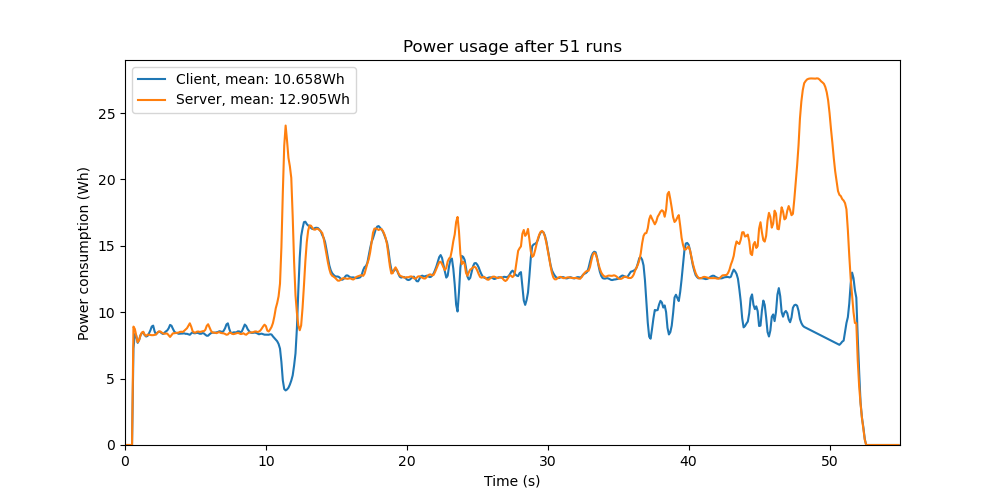
\includegraphics[width=\textwidth]{Thesis/Images/Means/mean_cheetah_resnet50.png}
%             \caption{Mean of running Cheetah with resnet50 51 times}
%             \label{fig:mean_cheetah_resnet50}
%         \end{subfigure}
%         \hfill
%         \begin{subfigure}[b]{0.5\textwidth}
%             \centering
%             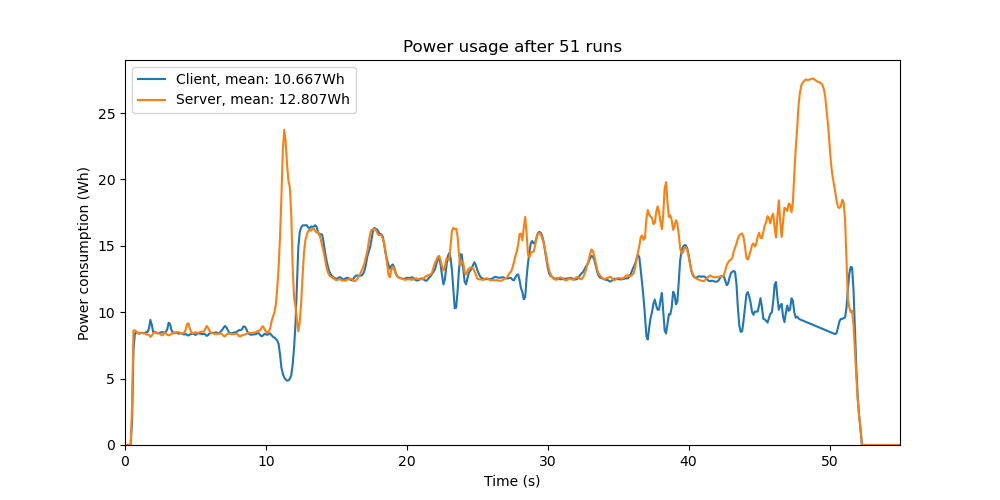
\includegraphics[width=\textwidth]{Thesis/Images/Means/mean_cheetah_sqnet.png}
%             \caption{Mean of running Cheetah with sqnet 51 times}
%             \label{fig:mean_cheetah_sqnet}
%         \end{subfigure}
     
%      \medskip
     
%      \begin{subfigure}
%         \begin{subfigure}[b]{0.5\textwidth}
%             \centering
%             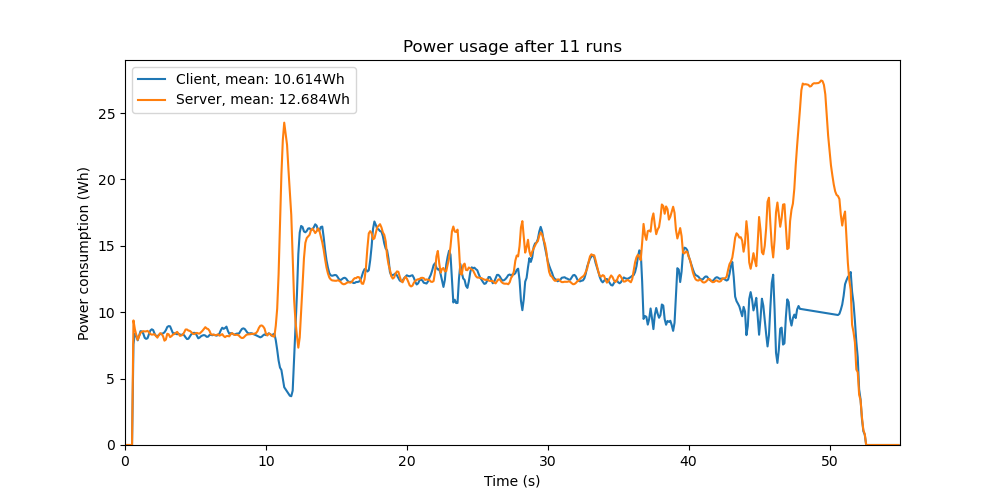
\includegraphics[width=\textwidth]{Thesis/Images/Means/mean_SCI_HE_sqnet.png}
%             \caption{Mean of running SCI_HE with sqnet 11 times}
%             \label{fig:fmean_SCI_HE_sqnet}
%         \end{subfigure}
%         \hfill
%         \begin{subfigure}[b]{0.5\textwidth}
%             \centering
%             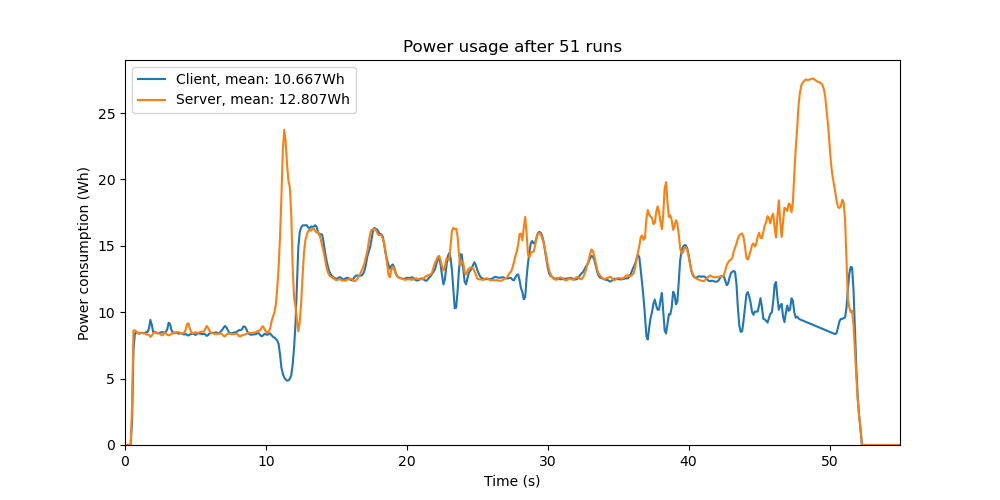
\includegraphics[width=\textwidth]{Thesis/Images/Means/mean_cheetah_sqnet.png}
%             \caption{Mean of running Cheetah with sqnet 51 times}
%             \label{fig:mean_cheetah_sqnet}
%         \end{subfigure}         
%      \end{subfigure}
     
%      \caption{Three simple graphs}
%      \label{fig:three graphs}
% \end{figure}

\subsection{Different devices}
\begin{table}
    \begin{adjustbox}{width=\columnwidth,center}
        \subfile{../Tables/Power_readings_client}
    \end{adjustbox}
    \caption{Power readings of running the Cheetah and $SCI_{HE}$ and limiting the bandwidth of the client.}
    \label{table:powerreadingsclient}
\end{table}

\begin{table}
    \begin{adjustbox}{width=\columnwidth,center}
        \subfile{../Tables/Power_readings_server}
    \end{adjustbox}
    \caption{Power readings of running the Cheetah and $SCI_{HE}$ and limiting the bandwidth of the server.}
    \label{table:powerreadingsserver}
\end{table}


\subsection{graphs}
\begin{figure}[hbt!]
    \begin{subfigure}{.475\linewidth}
            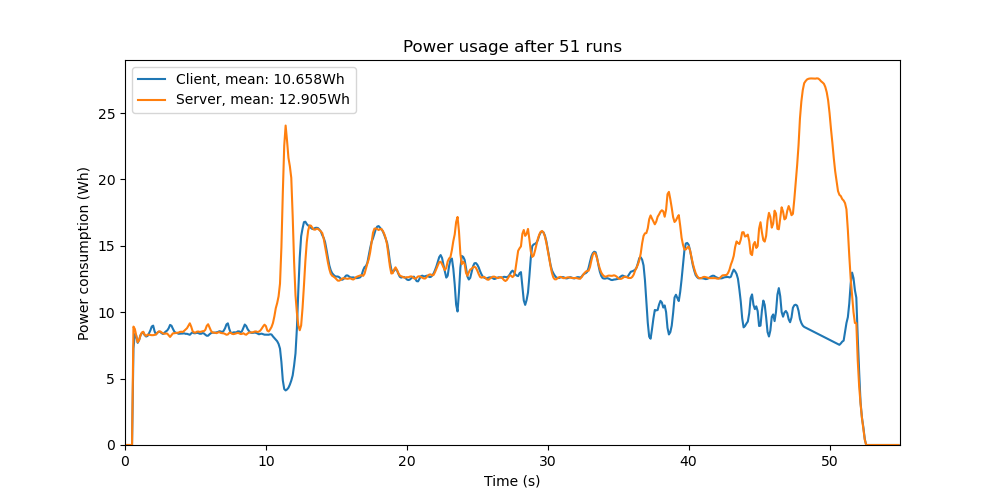
\includegraphics[width=\textwidth]{Thesis/Images/Means/mean_cheetah_resnet50.png}
            \caption{Mean of running Cheetah with resnet50 51 times}
            \label{fig:mean_cheetah_resnet50}
    \end{subfigure}\hfill % <-- "\hfill"
    \begin{subfigure}{.475\linewidth}
            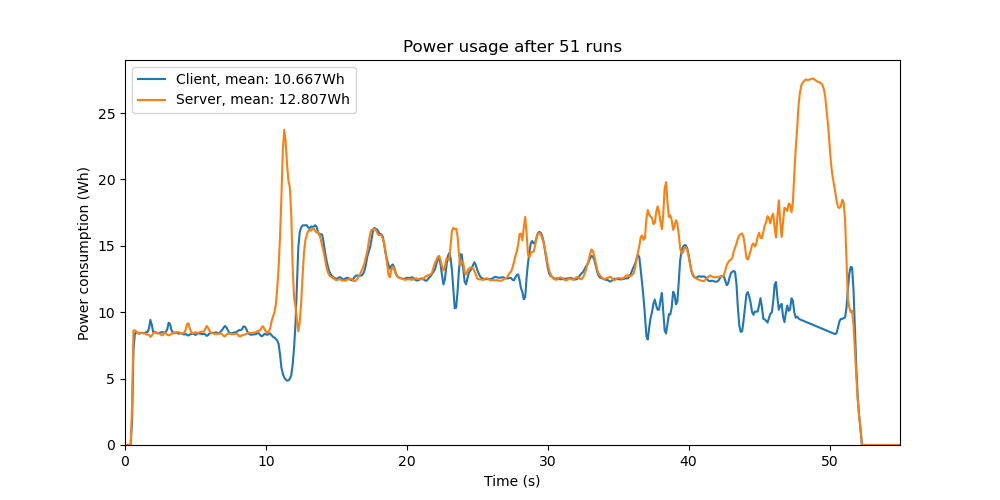
\includegraphics[width=\textwidth]{Thesis/Images/Means/mean_cheetah_sqnet.png}
            \caption{Mean of running Cheetah with sqnet 51 times}
            \label{fig:mean_cheetah_sqnet}
    \end{subfigure}

    \medskip % create some *vertical* separation between the graphs
    
    \begin{subfigure}{.475\linewidth}
            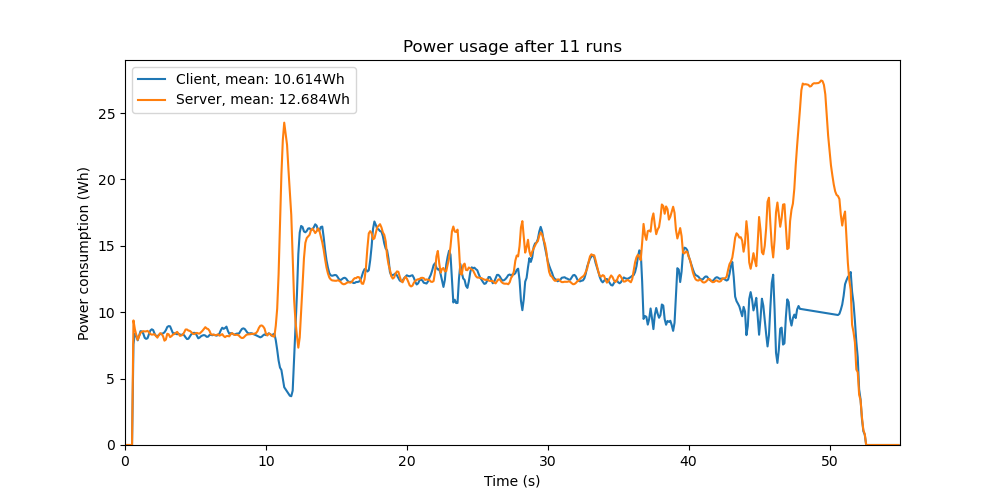
\includegraphics[width=\textwidth]{Thesis/Images/Means/mean_SCI_HE_sqnet.png}
            \caption{Mean of running SCI\_HE with sqnet 11 times}
            \label{fig:mean_SCI_HE_sqnet}
    \end{subfigure}\hfill % <-- "\hfill"
    \begin{subfigure}{.475\linewidth}
            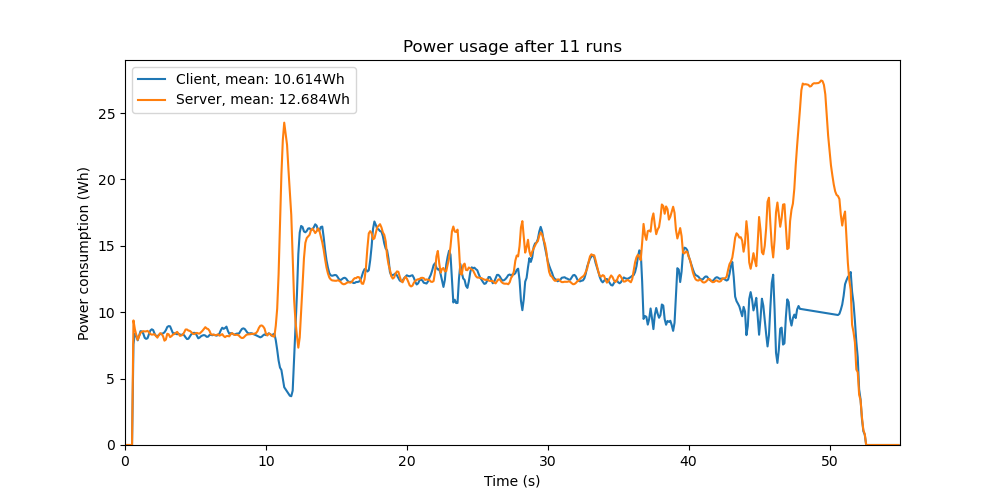
\includegraphics[width=\textwidth]{Thesis/Images/Means/mean_SCI_HE_sqnet.png}
            \caption{Mean of running SCI\_HE with sqnet 11 times}
            \label{fig:fmean_SCI_HE_sqnet}
    \end{subfigure}

    \caption{Four measurements doneA figure with four subfigures}
    \label{fig:4results}
\end{figure}

\begin{figure}[hbt!]
    \begin{subfigure}{\linewidth}
            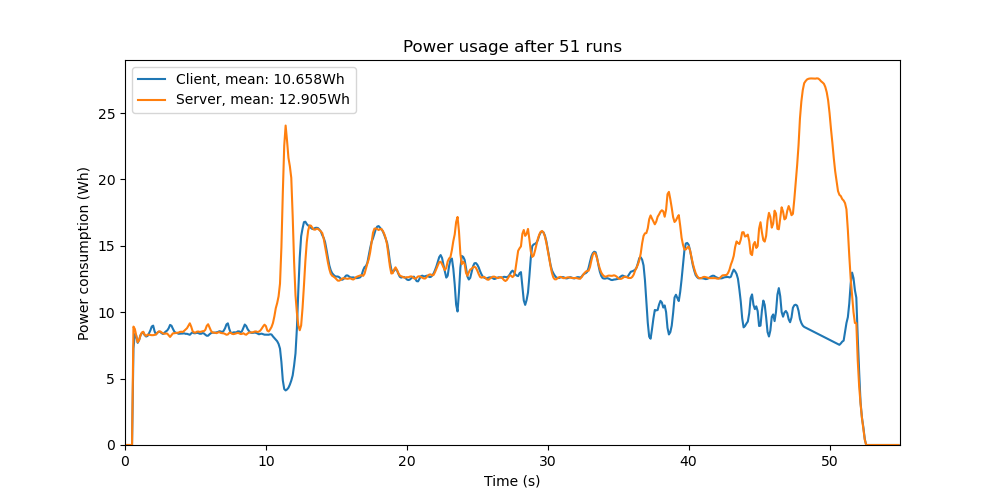
\includegraphics[width=\textwidth]{Thesis/Images/Means/mean_cheetah_resnet50.png}
            \caption{Mean of running Cheetah with resnet50 51 times}
            \label{fig:bmean_cheetah_resnet50}
    \end{subfigure}
    \begin{subfigure}{\linewidth}
            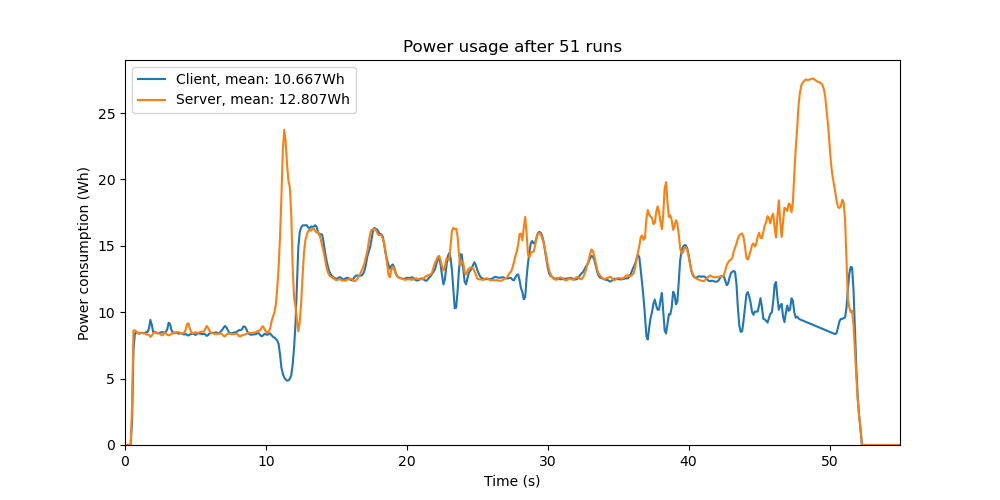
\includegraphics[width=\textwidth]{Thesis/Images/Means/mean_cheetah_sqnet.png}
            \caption{Mean of running Cheetah with sqnet 51 times}
            \label{fig:bmean_cheetah_sqnet}
    \end{subfigure}    
    \begin{subfigure}{\linewidth}
            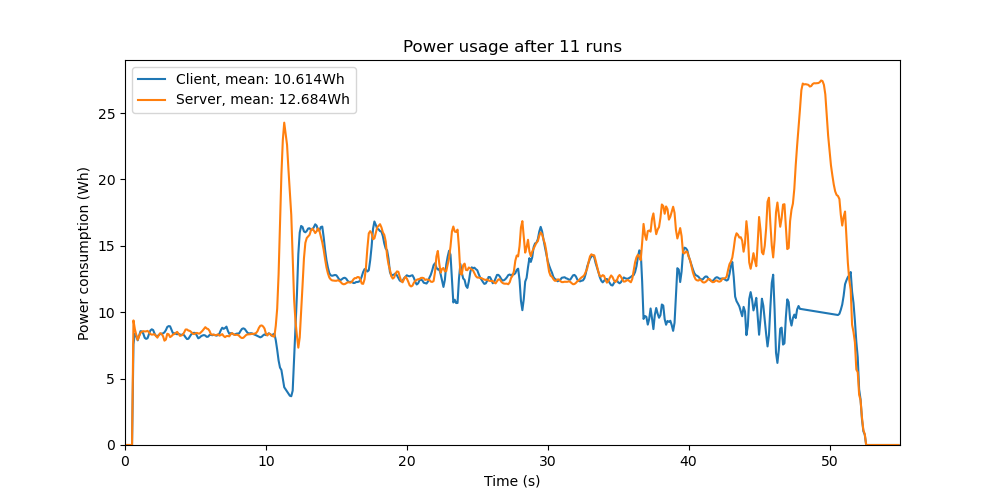
\includegraphics[width=\textwidth]{Thesis/Images/Means/mean_SCI_HE_sqnet.png}
            \caption{Mean of running SCI\_HE with sqnet 11 times}
            \label{fig:bmean_SCI_HE_sqnet}
    \end{subfigure}
    \begin{subfigure}{\linewidth}
            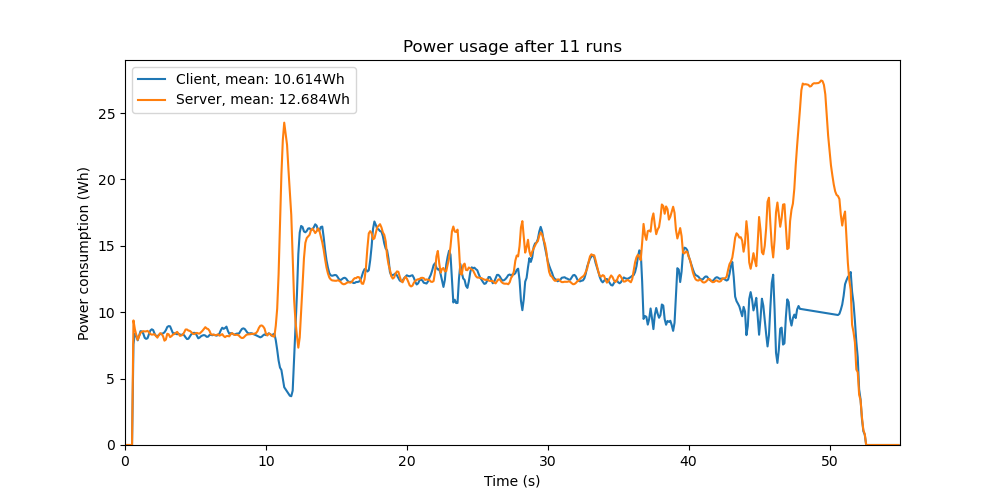
\includegraphics[width=\textwidth]{Thesis/Images/Means/mean_SCI_HE_sqnet.png}
            \caption{Mean of running SCI\_HE with sqnet 11 times}
            \label{fig:bfmean_SCI_HE_sqnet}
    \end{subfigure}

    \caption{Four measurements doneA figure with four subfigures}
    \label{fig:4results2}
\end{figure}

\noindent
Cross-references to subfigures \ref{fig:mean_cheetah_resnet50}, \ref{fig:mean_cheetah_sqnet} and \ref{fig:mean_SCI_HE_sqnet} and of figure \ref{fig:4results}.

% \begin{figure}[h!]
%     \centering
%     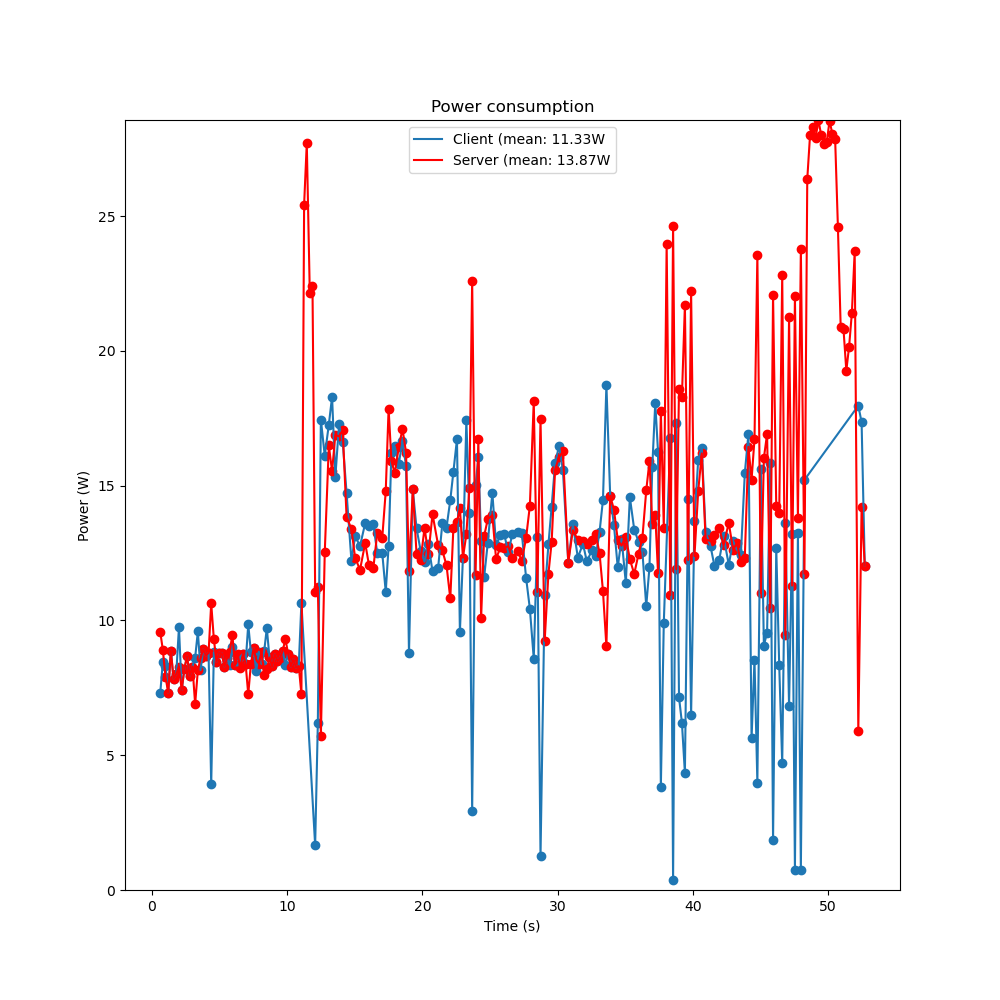
\includegraphics[width=\textwidth,height=\textheight,keepaspectratio]{cheetah-sqnet.png}
%     \caption{Running the SNNI cheetah on sqnet}
%     \label{fig:my_label}
% \end{figure}
% \newpage
% \begin{figure}[h!]
%     \centering
%     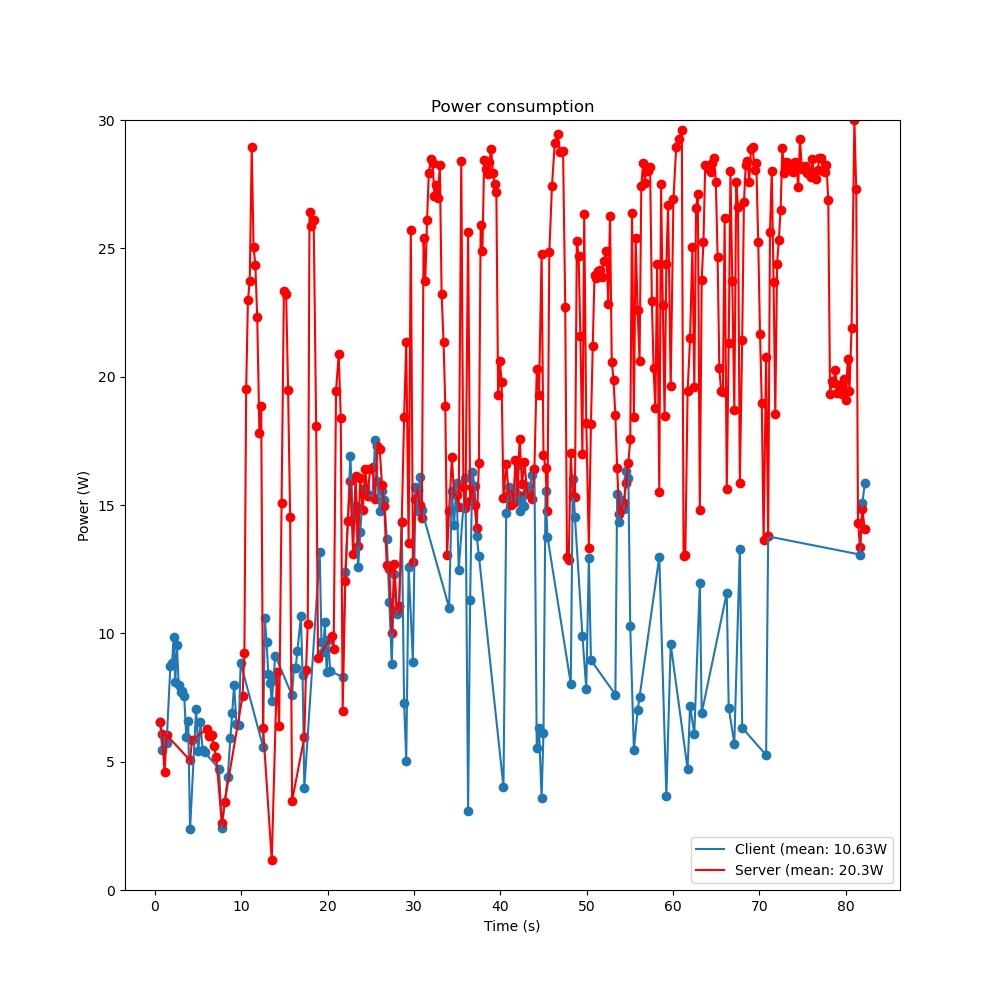
\includegraphics[width=\textwidth,height=\textheight,keepaspectratio]{SCI_HE-sqnet.png}
%     \caption{Running the SNNI CryptFlow2 on sqnet}
%     \label{fig:my_label}
% \end{figure}
\section{RQb, what are the differences on server and client side and what are the implications}
\end{document}
